\documentclass{article}

\usepackage{mathtools}
\usepackage{graphicx}
\usepackage{listings}
\usepackage{color}

\definecolor{mygreen}{rgb}{0,0.6,0} 
\definecolor{mygray}{rgb}{0.5,0.5,0.5} 
\definecolor{mymauve}{rgb}{0.58,0,0.82}

%Scala
\lstdefinelanguage{scala}{
  morekeywords={abstract,case,catch,class,def,%
    do,else,extends,false,final,finally,%
    for,if,implicit,import,match,mixin,%
    new,null,object,override,package,%
    private,protected,requires,return,sealed,%
    super,this,throw,trait,true,try,%
    type,val,var,while,yield},
  otherkeywords={=>,<-,<\%,<:,>:,\#,@},
  sensitive=true,
  morecomment=[l]{//},
  morecomment=[n]{/*}{*/},
  morestring=[b]",
  morestring=[b]',
  morestring=[b]"""
}

% Default settings for code listings
\lstset{frame=tb,
  language=scala,
  aboveskip=3mm,
  belowskip=3mm,
  showstringspaces=false,
  columns=flexible,
  basicstyle={\small\ttfamily},
  numbers=none,
  numberstyle=\tiny\color{mygray},
  keywordstyle=\color{blue},
  commentstyle=\color{mygreen},
  stringstyle=\color{mymauve},
  frame=single,
  breaklines=true,
  breakatwhitespace=true
  tabsize=3
}

\title{Metrics for code 'functional-ness' in Scala\\Dissertation proposal  }
\date{\today}

\begin{document}



\pagenumbering{gobble}
\maketitle

\vspace{30mm} %5mm vertical space

\begin{center}
Master Student Name: Alexandru Matei \par
Supervisor Name : Marius Minea \par
Dissertation Domain: Software engineering - Functional Programming
\end{center}

\vfill

\newpage
\tableofcontents
\newpage

\pagenumbering{arabic}
\section{Introduction}
Functional programming has started to gain more traction in the last years, thanks to the growing adoption of Scala and Haskell in the software industry; we can see that Google trends shows a rising interest in functional programming languages (see figure \ref{fig:google-rank}). \par

\begin{figure}[h!]
  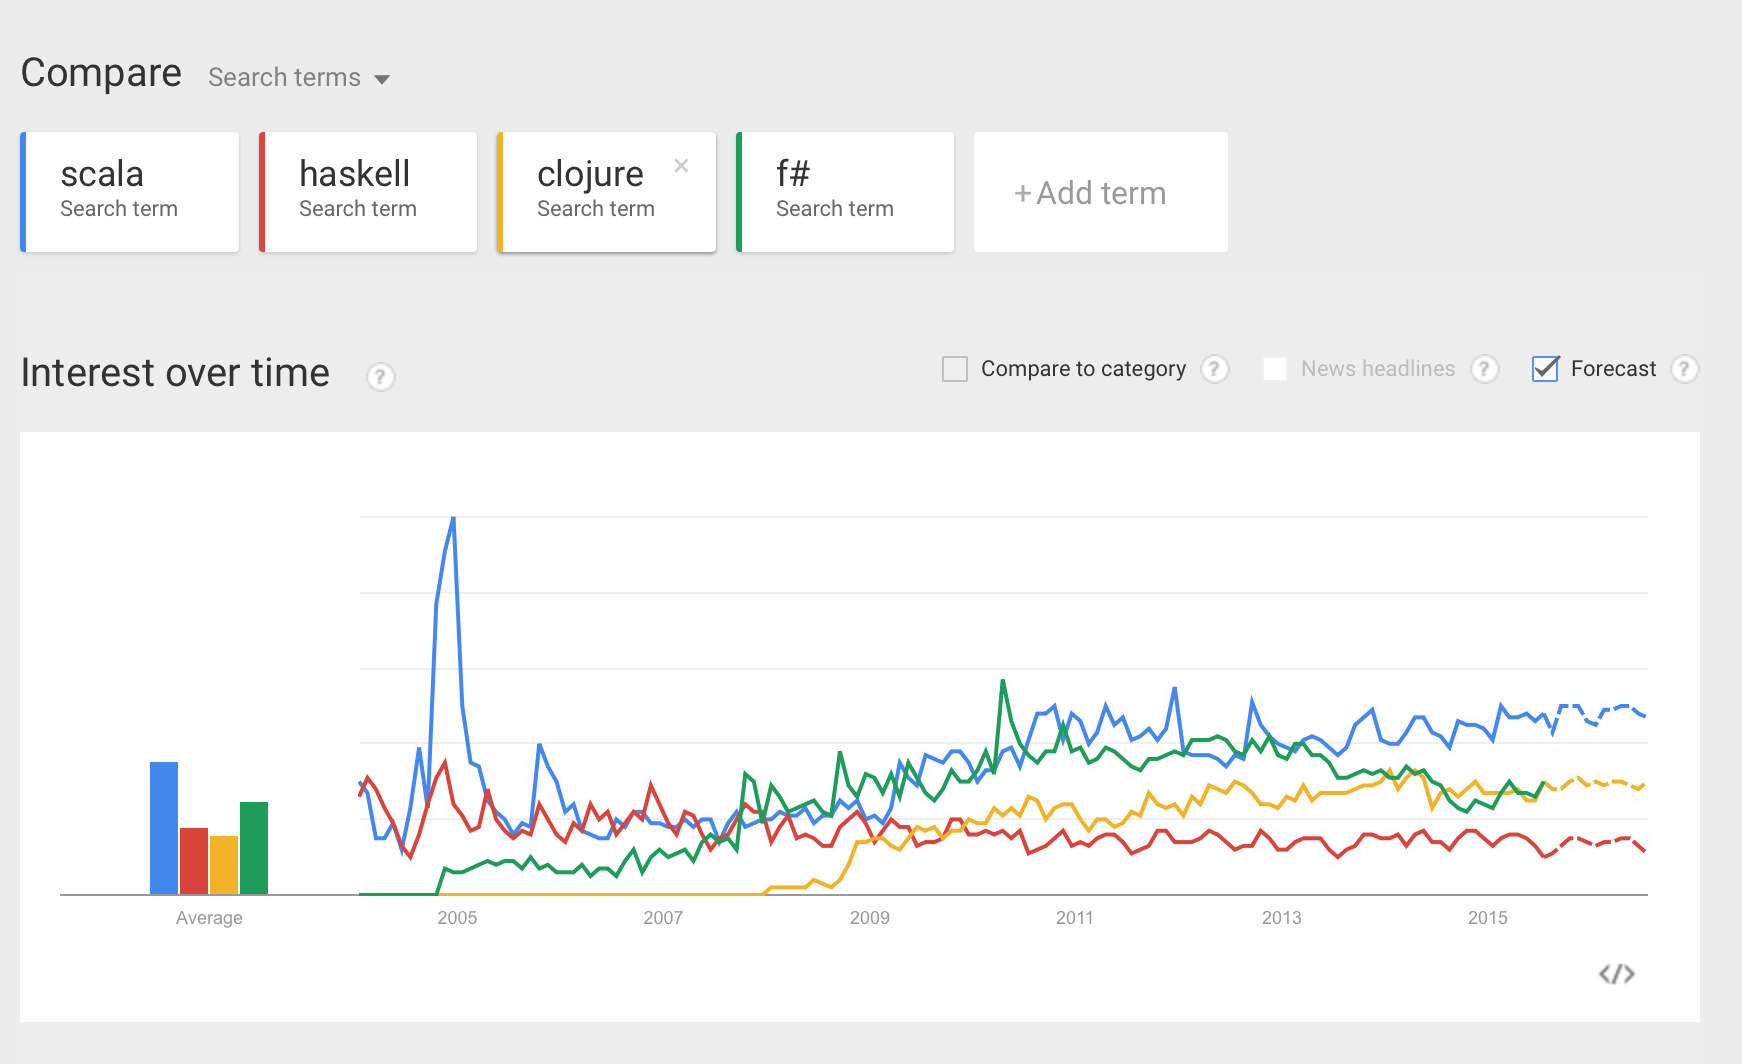
\includegraphics[width=\linewidth]{google-trends.png}
  \caption{Google search hits for programming languages - 2004 to July, 2015 }
  \label{fig:google-rank}
\end{figure}
There is a growing interest in functional programming languages, because of their expressive power and the possibility to reason about correctness of programs. There are claims on the readability of functional programs, for example: 'In many cases the functional programming style yields more elegant and comprehensible programs than the imperative programming style' (Springer \& Friedman, 1990) and 'Functional programming leads to programs which are exceptionally clear and concise and to the prospect of greatly increased software reliability and development speed' (Bailey, 1990). In a case study on the productivity of programming in a functional programming environment, some of these claims have been confirmed (Sanders, 1989).
Moreover, the learning of programming in a functional programming style should have advantages over learning in an imperative style (Springer \& Friedman, 1990; Bailes \& Salzman, 1989). \cite{DBLP:journals/infsof/BergB95} \par

Scala is one of the leading functional programming languages, over the last couple of years being adopted by large companies such as  Twitter(2009), Linkedin(2010), The Guardian, Foursquare. If we look at 'RedMonk Programming Languages Rankings'\cite{redmonk:1}, which is based on StackOverflow and Github analysis,  Scala occupies a worthy 14th position, being the first FP language in the top . \par

\begin{figure}[h!]
  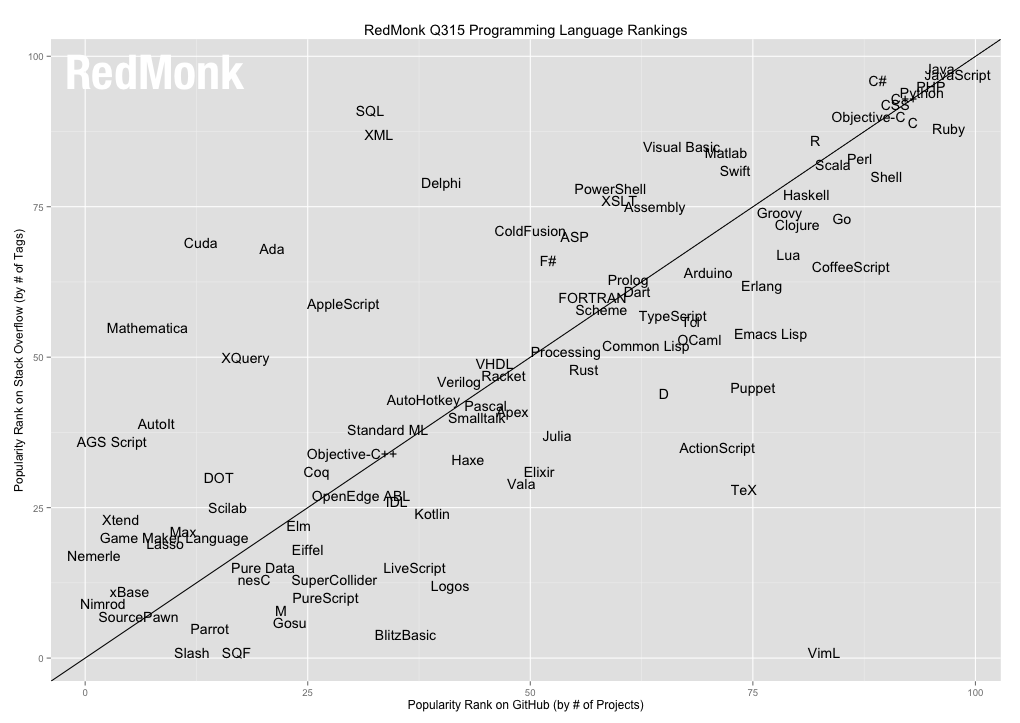
\includegraphics[width=\linewidth]{redmonk-rank.png}
  \caption{Redmonk rank of programming languages - June, 2015}
  \label{fig:redmonk-rank}
\end{figure}

One of its success factors is  Scala's compatibility with Java Virtual Machine hence code interoperability with Java, and the benefits that come along from  Java's well-established ecosystem.\par

 Another one might be that Massive Open Online Courses (MOOCs)  like Functional Programming in Scala \cite{scalastat:1} held  by the creator of Scala, Martin Odersky and Reactive Programming are one of the most popular online courses; the feedback from developers is really encouraging(see figure \ref{fig:interest}). \par

\begin{figure}[h!]
  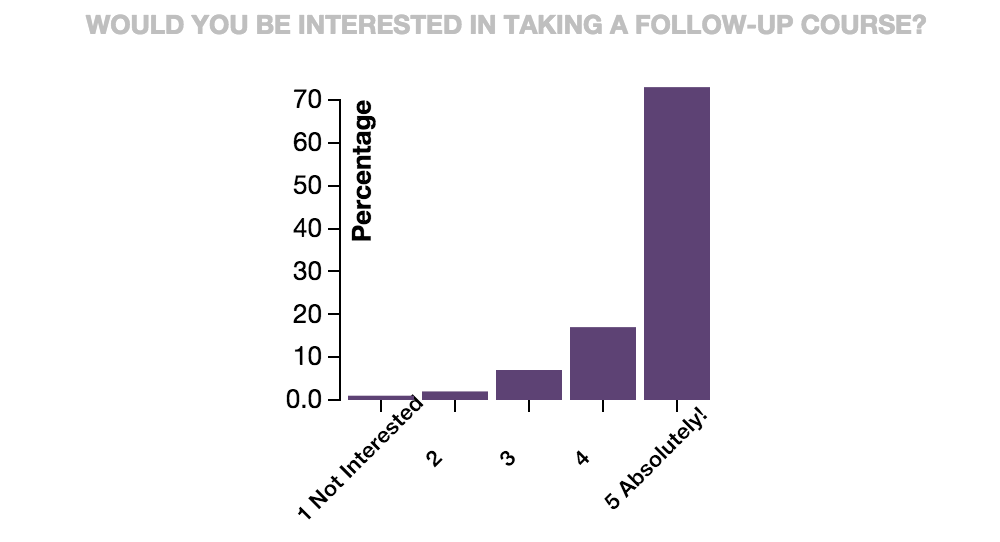
\includegraphics[width=\linewidth]{interest.png}
  \caption{Feedback FP in Scala course - interest in future courses on Scala (FP)}
  \label{fig:interest}
\end{figure}

Another reason why functional programming comes in handy nowadays is that multiprocessor architectures become ubiquitous and developers need to get more familiar with distributed and multi-threaded computing. Programming with shared state has proven to be  difficult to reason about and functional programming offers to save a lot of headaches by removing shared state from the equation and providing better concurrency abstractions (Futures, Actors). We should also consider  the exceptional distribution capabilities of map-reduce that functional programming offers. Although the programming paradigm was born more than 80 years ago, functional programming seems like a totally new way of thinking about software to modern day developers, having lots of secret gems left to be discovered. \par

\section {Problem statement}
Scala is a hybrid programming lanaguage combining both  functional and  object oriented elements \cite{scalalang:1}. Writing Scala code does not imply you are writing functional code;  there is no mechanism in the language that enforces a functional style of programming; so one can say they write code in Scala so they use functional programming when in fact their code base is entirely procedural. I was also put in such a position,  being one of the many  developers that switched from an Object Oriented language(Java /C\#/C++xs etc.)  to Scala. So how can one figure out if his Scala code follows the functional programming principles or not? The classic approach is to ask a functional programming expert for code review, if you are lucky enough to have access to such valuable resources. \par

The solution we propose is a set of metrics that should be able to quantify to what degree the code is making use of the functional paradigm. But what  qualifies a code as being functional? What are the characteristics of functional code? In the following section we will elaborate the main characteristics of functional programming languages.\par


\section {Theoretical Foundations}
First of all we need to establish the main elements of functional languages and we will do so by taking Scala as an example. Only then we can elaborate further on the metrics and decide which ones are to be considered for the study. \par


The question we will try to answer in this body of work is 'how much does a method use functional programming concepts?' The main elements we will look at are: immutability, referential trasparency, high-order functions, monads, laziness.

%We get to ask ourselves the following questions: `how much does a method uses functional programming concepts?` Does it contain only immutable data, so no shared state? Does it use higher order functions for data processing? Does a method use advanced features such as monadic comprehension? Does a method use functional-like constructs such as anonymous inner classes? \par

\subsection {Immutability}
If a variable/object is immutable then its value never changes. That is a useful guarantee if one plans on going concurrent: any such value can be safely shared amongst treads since the value is read-only. Another advantage is the reduced aliasing between different parts of the program; one can say that immutable objects are easier to reason about and also their API is straight forward because you don't need to reason about internal state changes - everything is transparent compared to mutable objects that introduce opaqueness in reasoning about their possible states at different moments of time . \par
Scala encourages immutability through case classes, which provide a syntatic sugar for creating immutable objects (data structures). Case classes are regular classes which export their constructor parameters and which provide a recursive decomposition mechanism via pattern matching.

\begin{lstlisting} 
abstract class Pet
case class Dog(name:String) extends Pet 
case class Cat(name:String) extends Pet
case class Hippo(name:String, weight:Int) extends Pet

//Decomposition
def printPetType(pet:Pet): String= pet match{
  case Dog => "it's a Dog"
  case Cat => "it's a Cat"
  case Hippo => "it's a Hippo"
}
\end{lstlisting}

By default, case classes ar immutable but one can change some of fields to be mutable, although it is not recommended.\par

Declaring a variable as a 'val' prevents it for being reassigned; still, this doesn't guarantee that the object it is reffering to is immutable. Best transparency is obtained with using both val's and immutable objects: this is the recommended approach also when dealing with concurrency. Scala provides both mutable and immutable collections that can be found in packages scala.collection.mutable and scala.collection.immmutable repectively. By default, Scala always picks immutable collections. 

\begin{lstlisting} 
val x = 4
x = 5 //Reasignment to val generates error
\end{lstlisting}


So, in order to create an immutable Scala object, it is necessary to have all the fields declared as vals + all the values to be immutable objects in turn. Case classes make it easier to accomplish that in as few lines of code as possible.

\subsection {Referential tranparency, pure functions}
An expression is referentially transparent (RT) if it can be replaced by its resulting value without changing the behavior of the program. This must be true regardless of where the expression is used in the program. Programming without side effects leads to referential transparency. An example:

\begin{lstlisting}
def f(x:Int)= x* 3
val z = f(3)
\\Now, whenever we use z in the code, we can safely
\\ replace it with f(3) without changing the result of the program
\end{lstlisting}

Pure functions evaluate to the same result given the same argument value(s) and  don't have any side effects. A definition combining both concepts can be found in 'Functional Programming in Scala' by Chiusano and Bjarnason : 'A function f is pure if expression f(x) is referentially transparent for all referentially transparent values x'.\par
Examples of pure functions in Scala include:
\begin{itemize}

 \item Methods on immutable collections such as map, drop, filter, take
 \item Methods like split, length on the String class
 \item Mathematical functions such as add, multiply \ldots
\end{itemize}
As a rule of thumb in Scala if a function has return type Unit, then most probably it has side effects and it is not pure. \par

A measure for the degree of referential transparency in a program can be expressed as:  \par
\begin{center}
\begin{math}
  RTI = \frac{ | \{ m \in M / Pure(m) \} | } { | M | }
\end{math}
\end{center}

Where RTI- Referential Transparency Index ,  M - set of all functions/methods of the software and  Pure(m) - predicate that says if a function is pure or not. In this case, a value close to 1 corresponds to improved referential transparency while one close to 0 says that the property is not satisfied at all. \cite{DBLP:conf/icse/MudduABP13}. Further study is needed on elaborating how the pure function should be defined. \par

\subsection {High-order functions}
The central concept of functional languages as pointed out by John Hughes \cite{DBLP:journals/cj/Hughes89} in 'Why Functional Programming Matters' is higher- order functions ; Hughes argues that when high order functions are combined with laziness techniques they greatly increase the modularity of software by providing novative ways (compared to other structured programming techniques) of 'gluing' modules together so programs can become more concise and easier to reason about. 

Before we begin talking about high-order functions we should first understand what does an order of a function mean:

\begin{itemize}
\item Order 0: Non function data
\item Order 1: Functions with domain and range of order 0
\item Order 2: Functions with domain and range of order 1
\item Order k: Functions with domain and range of order k-1
\end{itemize}

So order 0 is represented by numbers, lists, characters, etc. Order 1 are functions wich work with order 0 data. So order 1 data are the well known functions that every programming language supports. 
Functions with an order grater than 1 are callled higher-order functions and they fall at least in on of the following categories:
\begin{itemize}
\item they take other functions as parameters
\item they return a function as a result
\end{itemize}

Being able to pass functions as parameters and return them as results means that functions are first-class citizens and is one of the  core concepts that make a functional language.

An example is the following apply function written in Scala, which takes a function  and an integer as parameters and produces  a function as a result: \par

\begin{lstlisting} 
def apply(f: Int => String, v: Int) = f(v)
\end{lstlisting} 


Classical higher-order functions over lists :

\begin{itemize}
\item Mapping: Application of a function on all elements in a list
\item Filtering : Collection of elements from a list which satisfy a particular condition
\item Accumulation: Pair wise combination of the elements of a list to a value of
another type
\item Folding: Reducing a list over some function with accumulator
\end{itemize}
[http://people.cs.aau.dk/~normark/prog3-03/pdf/higher-order-fu.pdf]

A study about high-order functions metrics and their corelation with software modularity was also conducted by B. Muddu et. al. \cite{DBLP:conf/icse/MudduABP13}. The proposed metric was studying the coupling between high order functions in diferent modules. It might be useful to make use also of their modularity metric when assesing code functional-ness.\par 

\subsection {Monads}  \label{monads}
Monads are a central design pattern of functional programming. They've been successfully used to abstract over well known problems in programming \cite{Jones01tacklingthe}: non-determinism as expressed by list, time/ concurrency, mutable state (see IO Monad Haskell), exception handling, foreign language calls.

In Category Theory, a Monad is a functor equipped with a pair of natural transformations satisfying the laws of associativity and identity. In Scala, monads are just a parametric type M[T] with two operations, flatMap (or bind) and unit which also preserves associativity and identity. \par

\begin{lstlisting}
trait M[T]{
  def flatMap[U](f:T=>M[U]): M[U]
}

def unit[T](x:T): M[T]
\end{lstlisting}

\subsection {Lazy evaluation}
Lazy evaluation or call-by-need is the opposite of eager evaluation(call-by-value) and it is an evaluation strategy which delays the evaluation of an expression until it is needed and only then computes the result and caches it for further evaluations. \par
One advantage is the memory saving due to postponing the evaluation but it comes with a performance cost: you get faster intialization but later (when evaluation occurs) you suffer a performance penality.\par

Scala supports laziness by introducing the lazy keyword and call by name parameters. By default it supports strict evaluation in contrast with Haskell which is lazy by default.

\begin{lstlisting}
lazy val product = 100 * 30 // not evaluated
println(product.toString) // evaluated 


object Test {
   def main(args: Array[String]) {
        delayed(time());
   }

   def time() = {
      println("Getting time in nano seconds")
      System.nanoTime
   }
   def delayed( t: => Long ) = {
      println("In delayed method")
      println("Param: " + t)
      t
   }
}

\end{lstlisting}

\section {State of the art - Literature study}
In the first section we talked about elaborating a series of metrics, in order to asses one's code functional-ness but we didn't have the opportunity to provide a proper definition for the concept of a metric and it's existing state of affairs in software industry. An easy definiton would be that metrics offer a quantitative measure of a software property. 

\subsection{Metrics overview and their use in FP languages}

\textit{"When you can measure what you are speaking about and express it in numbers, you know something about it; but when you cannot measure it, when you cannot express it in numbers, your knowledge is of a meagre and unsatisfactory kind: it may be the beginnings of knowledge but you have scarcely in your thoughts advanced to the stage of Science." (Lord Kelvin)}\par

A metric is a measurement function, and a software quality metric is "a function whose inputs are software data and whose output is a single numerical value that can be interpreted as the degree to which software possesses a given attribute that affects its quality'' \cite{Kaner04softwareengineering}. To some extent, metrics could be regarded as compiler warnings, signaling that a part of your code needs more testing. Software metrics are used in Software Engineering for helping with software development activities such as testing and refactoring, performance optimization, debugging, cost estimation, etc. Some common software metrics include : source line of code (LOC), number of functions, cyclomatic complexity, code coverage, cohesion, coupling. \par

Study of software metrics has been an active area of research since early 70' targeting mostly object oriented and imperative languages \cite{RyderT05:TFP_2005_Intellect}; as for functional languages, the number of published papers is not the numoerous; some of the prior work on metrics for functional languages was started almost 20 years ago by K. van den Berg in 1995 \cite{DBLP:journals/infsof/BergB95} who proposed a set of metrics for evaluating code complexity of Miranda functional programming language and Harrison which studied code modularity for SML \cite{eps250597}; 10 years later, Ryder and Thompson proposed some metrics for Haskell \cite{RyderT05:TFP_2005_Intellect} whereas  Muddu et. al. developed metrics for Scala \cite{DBLP:conf/icse/MudduABP13}. We can corelate the few number of papers on FP with the fact that FP does have yet such large adoption in software industry compared to object oriented and imperative languages.  \par

\subsection{Static analysis of functional programs- K. van den Berg}
K. van den Berg performed a coparison study regarding code coprehensibility of program code: how easy is it to a developer to read and understand a program in order to find and fix some errors or to adapt to changing requirements. The languages that were studied are Pascal and Miranda, the first being the representative for `imperative languages`, the last representing `functional languages`. One of the metrics he chose to use are Halstead and McGabe's, which were adapted for both programming paradigms. \par

Halstead metrics can be expressed as :

\begin{itemize}
\item $\eta_1$ - the number of unique operators \par
\item $\eta_2$ - the number of unique operands \par
\item $N_1$ - the total number of operators \par
\item$N_2$ - the total number of operands \par
\item$\eta_2'$ - the number of different input/output parametes \par
\end{itemize}

Using this terminology, one can define the following:\par
\begin{itemize}
\item $\eta = \eta_1 + \eta_2 $ - the vocabulary of a program \par
\item $N = N_1 + N_2 $ - the length of a program as total number of tokens \par
\item $V = N * \log _2 \eta $ - the size of a program (volume) \par
\item $V' = (2 + \eta_2')*\log_2(2 + \eta_2')$ - the potential volume of a program \par
\item $L = V' / V $ - program level or level of implementation \par
\item $E = V / L $ - effort to generate a program
\end{itemize}

McGabe's metrics for ciclomatic complexity focus on the decision structure of a program. The program is viewed as a decision graph G, having a unique entry and exit point. Every edge in the graph represents a decision branch while every node is a decision point. This metric is related to the difficulty of testing a program. The metric can be expressed as :
\begin{itemize}
\item $e$ - the number of edges in the program graph \par
\item $n$ - the number of nodes \par
\item $v(G) = e - n + 2$ - the ciclomatic complexity number
\end{itemize}

The study of Curtis (1981) shows empirical evidence that the complexity metrics of McCabe and Halstead relate to the psychological complexity, as expressed in the difficulty in understanding and modifying software. The relation between syntactic complexity and cognitive complexity has been investigated by Khalil \& Clark (1989). Shen, Conte \& Dunsmore (1983) give a critical review of Software Science. They show that the effort E, as defined by Halstead, correlates with the understandability of programs. . \cite{DBLP:journals/infsof/BergB95}. \par

What we take for our study of  K. van den Berg's paper is the adoption of Halstead and McGabe's metrics for functional programs. Using these metrics we could asses the complexity of our functional program and we could correlate it with other metrics. 

\subsection{Comparing Programming Paradigms: an Evaluation of Functional and Object-Oriented Programs - R.Harrisson et. al.}
Another study that targeted a comparison between imperative and functional languages was that of R. Harrison et. al. \cite{eps250597} . After comparing C++ with SML they reached to the conclusion that SML code is more reusable then C++ but it also takes longer to be tested; one of the reason why testing takes so much was that SML needed to be reloaded before tests were run. \par

Their approach was to find a correlation between development metrics such as : number of know errors (KE), time to fix errors(TKE), number of modification requests (MR), time to implement modifications(TMR) and a subjective assement of complexity(SC) and some code metrics; the code metrics of their choice where the number of non-commmented lines (ncsl), number of distinct functions ($N'$), number of distinct library functions (L), number of distinct domain functions(D), depth of function hierarchy chart, number of function declarations, number of function definitions. \par

A nice metric for reusability that we can further use in our pursue of code functional-ness is reusability expressed as the ratio between number of library functions called ($L$) and number of distinct functions ($N'$): $R = L / N'$. \par

\subsection{Software Metrics: Measuring Haskell - Chris Ryder and Simon Thompson}
In their paper, Ryder and Thompson propse a collection of software metrics of Haskell programs. They can be devided into:
\begin{itemize}
\item pattern metrics - measuring pattern matching complexity
\item distance metrics - scoping length, size, etc.
\item callgraph attributes 
\item function attributes
\end{itemize}

\subsubsection{Pattern metrics}
\begin{itemize}
\item Pattern size (PSIZ) - number of components of the pattern's abstract syntax tree (AST)
\item Number of pattern variables (NPVS) - pattern variables represent new identifiers that are added to the program scope
\item Number of overriden/overrided pattern variables (NOPV) - one can mistakely override some variables already presented in scope when pattern matching
\item Number of pattern constructors (PATC) 
\item Number of wildcards used (WILD) -  wildcards may convey information about the structure of items in the pattern, e.g. the position of constructor arguments.
\item Depth of nesting - how many patterns are nested in one pattern matching expression e.g. Car(Wheels(Michelin(\_)), Motor(Wolkswagen(100CP(\_))))
\subitem Sum of the dept of nesting (SDNP)
\subitem Maximum depth of nesting (MDNP)
\end{itemize}

\subsubsection{Distance metrics}

\begin{itemize}
\item Number of new scopes (NNS) - measure the distance between declaration and usage and how many new scopes were introduced in between; this should indicate how complex the name-space is at that use
\item Number of declarations brought into scope (NDBS) - how many declarations have been introduced into the name-space \ref{fig:scope-distance}

\begin{figure}[h!]
  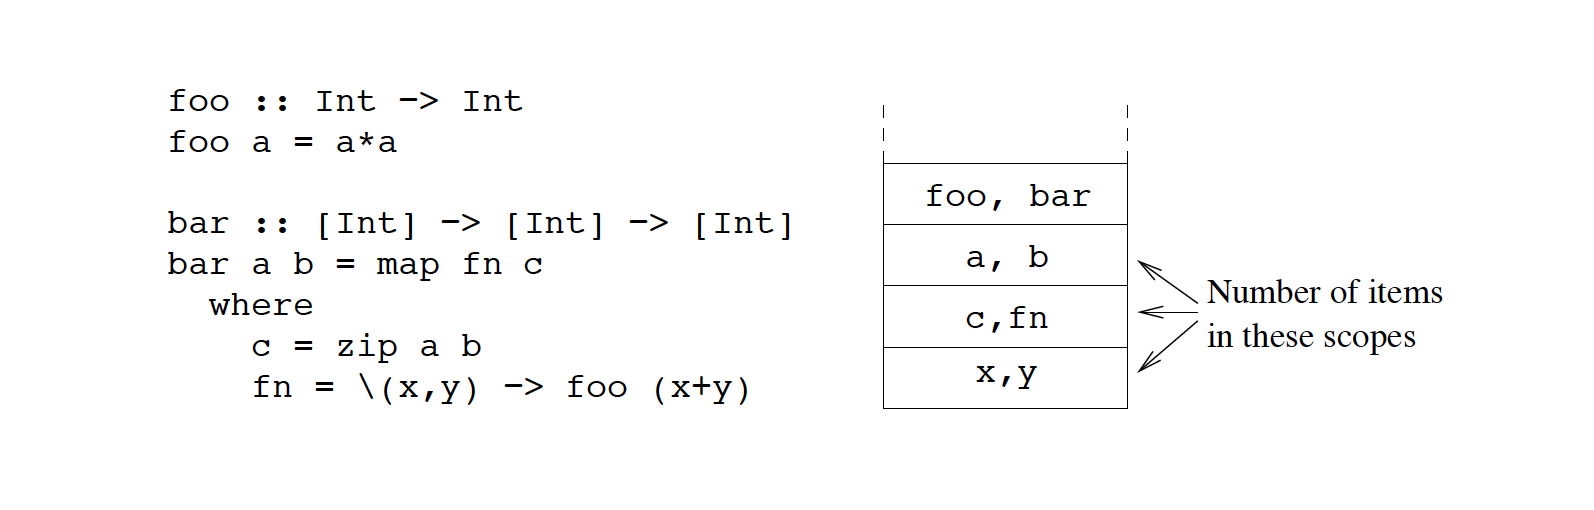
\includegraphics[width=\linewidth]{scope-distance.png}
  \caption{Measuring distance by the number of declarations brought into scope}
  \label{fig:scope-distance}
\end{figure}

\item Number of source lines - “spatial” distance in the source code; measuring the distance between the use of an identifier and the import statement that brings it into scope, plus the distance between the declaration and the start of the module in which it is defined. \ref{fig:scope-measure}

\begin{figure}[h!]
  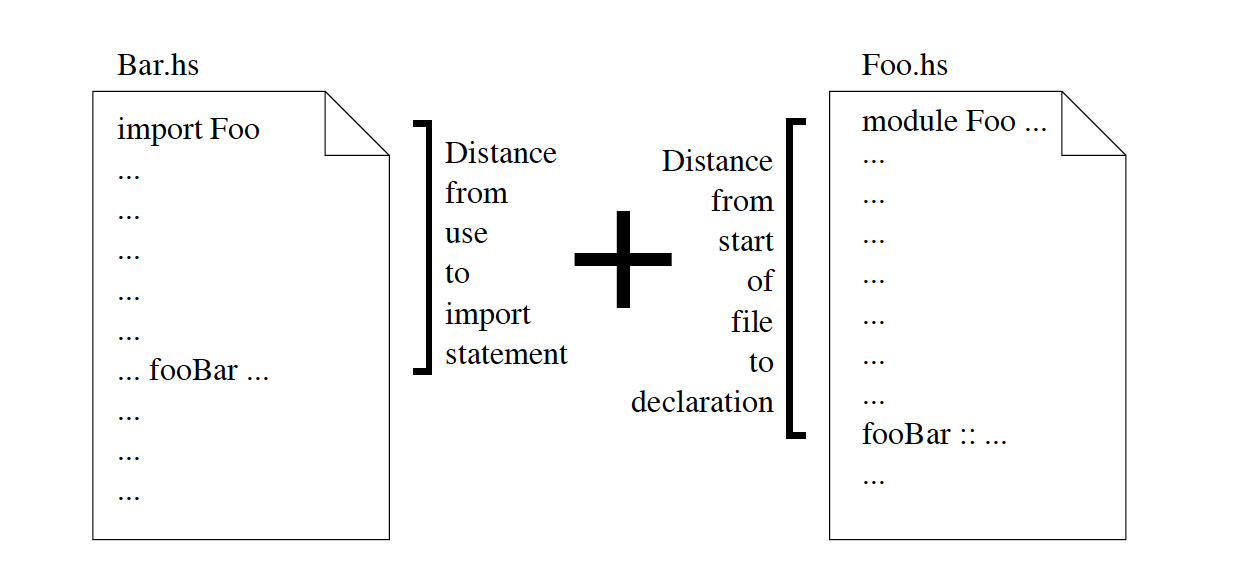
\includegraphics[width=\linewidth]{scope-measure.png}
  \caption{Measuring distance between use of identifier and import statement }
  \label{fig:scope-measure}
\end{figure}

\item Number of parse tree nodes - count the number of parse tree nodes on the path between two points of the parse tree

\end{itemize}


\subsubsection{Callgraph attributes}
\begin{itemize}
\item Strongly connected component size (SCCS) - A strongly connected component (SCC) is a subgraph in which all the nodes (functions) are connected (call) directly or indirectly to all the other nodes; as the size of the SCC increases, the number of changes is likely to increase as well, because a change to a single function may cause changes to other functions in the SCC. SCCS is a measure of coupling, similar to imperative and OO coupling metrics such as the Coupling between object classes (CBO), still it measures indirect coupling between functions, not objects (CBO)
\item Indegree (IDEG) - The indegree of a function in the callgraph is the number of functions that use it. Functions with high IDEG values may be more important, because they are heavily reused in the program and therefore changes to them may affect much of the program.
\item Outdegree (OUTDEG) - The outdegree of a function in the callgraph is the number of functions it calls.
\item Arc-to-node ratio (ATNR) - The arc-to-node ratio is a useful indicator of how “busy” a graph is.
\item Callgraph Depth (CGDP)
\item Callgraph Width (CGWD) - The subgraph of a function may be cyclic but can be transformed into a tree by breaking its cycle \ref{fig:subgraph-brake}
\begin{figure}[h!]
  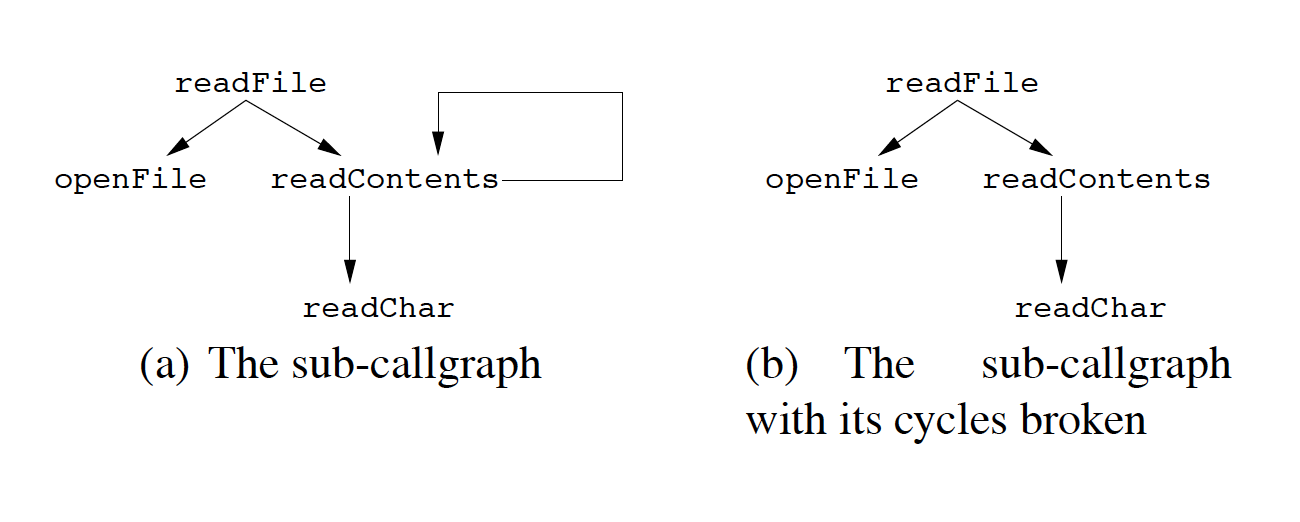
\includegraphics[width=\linewidth]{subgraph-brake.png}
  \caption{Breaking a cycle of a subgraph}
  \label{fig:subgraph-brake}
\end{figure}

\end{itemize}

\subsubsection{Function attributes}
\begin{itemize}
\item Pathcount (PATH) - Pathcount is a measure of the number of logical paths through a function
\item Operators (OPRT) -number of function operators
\item Operands (OPRD) - number of function operands \newline 
The last two are a measure of function size. A large function is more likely to be complex than a small one.
\end{itemize}

In order to validate their metrics, Ryder and Thompson performed analysis over a program's lifetime bug fixes and refactorings. Their conclusions: OUTD metrics is correlated with the number of changes and also SCCS has a significant correlation. They also studied cross correlation between metrics presented above \ref{fig:cross-correlation}.

\begin{figure}[h!]
  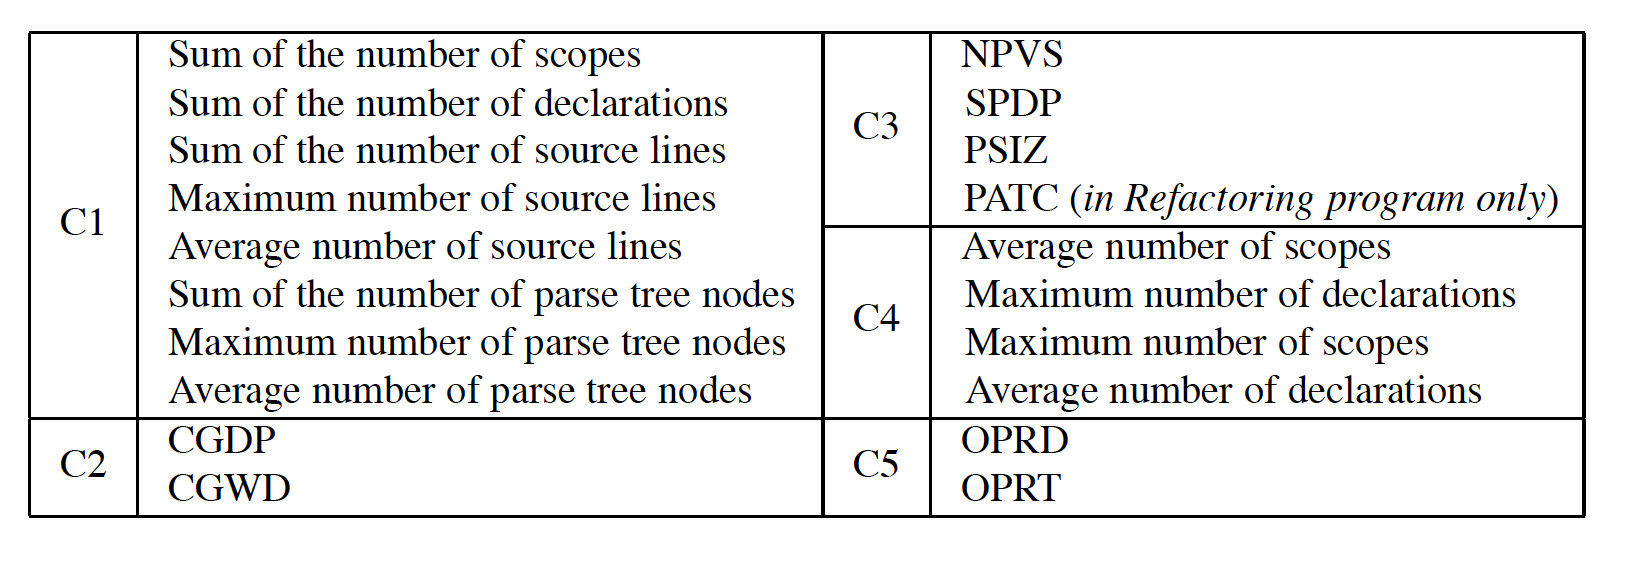
\includegraphics[width=\linewidth]{cross-correlation.png}
  \caption{Strongly correlated metrics}
  \label{fig:cross-correlation}
\end{figure}

\subsection{Metrics for modularization assessment of Scala and C\# systems - B. Muddu et. al.}
Basavaraju Muudu et. al. \cite{DBLP:conf/icse/MudduABP13} propose a series of metrics for Scala that target modularity with respect to Functional Programming features like : referential transparency, functional purity, first order functions and also Object Oriented features such as inheritance.


\subsubsection{Notation}

\begin{itemize}
\item S represents the software system, which consists of a series of modules $\varrho= \{ p_1,p_2,..,p_N \}$ and where $p_i$ is a system module, $1<=i<=N$
\item C - the set of all classes in the system S, C(p) -> the subset of all the classes containde in module p
\item M - the set of all methods/functions in the system S; M(c) is the subset of methods defined in class $c \in C$ and M(p) - the subset of functions defined in module $p \in \varrho$
\item NC(m1,m2) - number of calls from m2 to m1
\item FOC(m1,m2) - true if m2 is used as a parameter in a function call within m1; NFOC(m1,m2) counts the number of such calls
\item InUse(m) - true if a method is called during program execution 
\item Pure(m) - true(1) if m is a pure function
\end{itemize}

\subsubsection{Referential trasparency metrics}

\begin{itemize}
\item Referential Transparency Index (RTI) - referential transparency can be expressed as:  

\begin{center}
\begin{math}
  RTI = \frac{ | \{ m \in M / Pure(m) \} | } { | M | }
\end{math}
\end{center}

\item Intermodule Referential Transparency Index (IRTI) - measure the proportion of the calls in a certain module to methods in other modules which are pure over all the intermodule calls

\begin{center}
$ IRTI(p) = \frac {\sum_{m \in M(p)} \sum_{m' \in  {M - M(p)}} NC(m,m') \times Pure(m')} {\sum_{m \in M(p)} \sum_{m' \in {M - M(p)}} NC(m,m')} $
\end{center}

For the entire system: 

\begin{center}
$ {IRTI(S) = \frac {1} {|\varrho|} \sum_{p \in \varrho} IRTI(p)} $ 
\end{center}
\end{itemize}

\subsubsection{First order function metrics}
\begin{itemize}
\item Intermodule First Order Index 1 ($IFOI_1$) - determines the proportion of the methods in a certain module which make first order function calls to methods in another module

\begin{center}
  $IFOI_1 (p) = 1 - \frac {|\{m \in M(p) \mid \exists_{m' \in M} FOC(m,m') \and Mod(m') \neq p \}|} {|\{m \in M(p) \mid \exists_{m' \in M} FOC(m,m')\}|} $ 
\end{center}

\item Intermodule First Order Index 2 ($IFOI_2$) measures the proportion of out-side first-order-calls used by the current module

\begin{center}
  $IFOI_2 (p) = 1 - \frac { | \{m' \in M \mid \exists_{m \in M} FOC(m,m') \and Mod(m') \neq p \} | } { |\{ m \in \{ M - M(p) \} \exists_{m' \in M} FOC(m,m')   \}| }$
\end{center}

\item Intermodule First Order Index 3 ($IFOI3$) - measures the proportion of the other modules whose methods are called upon in a first order way by current module’s methods

\begin{center}
  $IFOI_3 (p) = 1 - \frac {| \{ p' \in \varrho \mid \exists_{m' \in M(p')} FOC(m,m') \and p' \neq p  \}|} {|\varrho| - 1} $
\end{center}

\item Intermodule First Order Index (IFOI)
\begin{center}
  $IFOI(p) = min(IFOI_1,IFOI_2,IFOI_3)  $ \\ 
  $IFOI(S) = \frac {1} {\varrho} \sum_{p \in \varrho} IFOI(p)$
\end{center}

\item Pure First Order Function Index (PFOI) - measures the proportion of all the first order calls which are to pure methods

\begin{center}
  $PFOI  = \frac { \sum_{m \in M} \sum_{m' \in M} NFOC(m,m') \times Pure(m') } { \sum_{m \in M} \sum_{m' \in M} NFOC(m,m') } $
\end{center}

\item Intermodule Pure First Order Function Index (IPFOI) - the ratio between the first order calls to pure methods residing in another module over all the first order calls done
\begin{center}
  $IPFOI(p) = \frac { \sum_{m \in M(p)} \sum_{m' \in \{M-M(p) \}} NFOC(m,m') \times Pure(m') } { \sum_{m \in M(p)} \sum_{m' \in \{M - M(p)\}} NFOC(m,m') } $ 
\end{center}

System wide:

\begin{center}
$IPFOI(S) = \frac 1 {|\varrho|} \sum_{ p \in \varrho } IPFOI(p)  $
\end{center}

\end{itemize}


\subsubsection{Module discovery}
They give the following definition for a module: ' A module is a logical collection of related files which can be modified and tested independently. A well modularized system will have low inter-module coupling and high intra-module cohesion. It helps the designers to add new modules easily.'\cite{DBLP:conf/icse/MudduABP13}. As one can see, this definition does not imply an exact rule for discovering  modules, so the system can contain a variable number of modules, depending how one delimits a module. \par
The technique they chose to use for delimiting system modules  was Modularizing by  Inverse-Depth heuristic, which is based of the project's file directory structure; they start at the source root folder and compute for each branch the maximum depth; then starting from the bottom up, they assign a module up to a certain depth; in their study, they use inverse depth of 1 for selecting modules, arguing that these are the closest approximation to actual logical modules. We would like to try other modularization techniques: package based, SBT (Scala Build Tool)  modularization and relate them to our problem: establishing code functional-ness: would a good 'functional-ness' value for our proposed metric lead also to improved modularity?.\par
The authors also suggest a metric that penalizes the coupling of multiple modules through inheritence and trait implementation. We should try working with penalization metrics, that count either the presence of absence of a feature in the source code.

\subsection {Combining Functional and Imperative Programming for Multicore Software: An Empirical Study Evaluating Scala and Java}
Pankratius et. al. performed a comparison study on Scala and Java's parallel programming features and performance \cite{Pankratius_combiningfunctional}. Their study shows that writing Scala code results in fewer lines of code than in Java and it preserves the application performance overall. One problem they notice is that Scala's support for parallelism is not as good as Java's. On top of that, Scala seems to require more debugging in testing effort which is quite problematic. One would expect that functional code should lead to fewer, easy to test lines of code. \par

An interesting point in their conclusion is that the top software developers participating in their study wrote a hybrid program, half functional and half imperative. So what would be the right balance between FP and imperative for a 'good Scala program'? \par

In order to make a distinction between functional and imperative programming, the authors classifed key language constructs in imperative ones: var, object, array, while, for,
abstract, import java and into functional ones: val, list, map,filter, flatmap, foreach, ::: (list concatenation),:: (list cons operator). That way they could asses how much of the code uses functional keywords and much is imperative.  Of course this measurement is a basic one but it is a good place to start from in our pursuit of code functional-ness.

\subsection{ Literature conclusion}

The biggest problem with code metrics is not the definition of new ones but the extraction of  meaningful information from them;code metrics without semantics attached to them are just plain numbers; we need to corelate them to some process development metrics and this is the hardest part, since process activities are difficult to cuantify; most of the research in FP metrics is targeting maintanability, code quality. We would like to see how functional property metrics impact refactorings; is there a way to detect 'functional code smells'?.  \par

Given previous papers on measuring programs written in functional languages, we would like first to find means to measure (if possible) all functional properties described in the previous chapter and try to relate them to both code quality and possible refactorings; it would be nice to study if some object-oriented structres could be restructred to FP patterns. Huiqing Li propose a refactoring tool for functional programms written in Haskell\cite{Li:2003:TSR:871895.871899}; starting from here, we can imagine corelating our metrics with possible refactorings suggestions, of course, this goal is rather ambitious but it's worth a little more study on the matter.

\subsection {Static analysis tools for Scala}
There are already a couple of static analysis tools written for Scala : ScalaStyle, ScapeGoat, Wart remover, Linger and Scala Abide. These tools are looking possible errors that might appear in Scala code and also checks for a certain style of coding. Some of the checks they perform are: identation, illegal imports, multiple declared strings, null appearances, redundant if statements, cyclomatic complexity, unreachable catch statements, unexpected recursive definitions, unassigned variables, shadowing etc. \par

Some metrics that could turn out to be useful for our study are  the presence, absence of vars and cyclomatic complexity; ScalaStyle checks that classes and objects do not define mutable fields and that functions do not define mutable variables (VarFieldChecker, VarLocalChecker) \cite{scalastyle} and it also has a metric for cyclomatic complexity. At least from an implementation perspective it would be worthwhile to take them into account.\par

\section{Conclusions and Future work}
In this paper we've looked at the main characteristics defining functional code and discussed the existing body of work regarding metrics inside functional languages. The state-of-the-art leaves a lot of room for new investigation to detect flaws. This is will be the main purpose of our research.

The leading question of this work as presented in  section 1  is  'How can we determine the degree of code "functional-ness" '? What code patterns can we define as not being functional, how can we detect them and what can we do about them? \par

In most practical situations we cannot give binary answers on the functional-ness of a codebase. Instead we will make use of metrics to quantify this aspect. The first step will be to conduct a study on which functional elements can be measured and which not. We will need to establish the granularity of what we want to investigate: intra-method level, inter-method, class-level. Afterwards, we will design a series of metrics to measure functional properties of the program. \par

The second step will be to implement a plugin in one of the main technologies used in the Scala ecosystem to make these measurements.\par

The third step will be to apply our plugin against a substantially large codebase and evaluate its effectiveness in detecting code flaws and ``bad smells''. Our theoretical model should be complete enough to give reasons and refactoring suggestions for these when we detect them.


\subsection {Coordinator guidance}

\subsubsection {Problem definition}
Cum ziceam, intrebarea cheie e la ce folosesti aceste metrici.

Punerea problemei in sec. 2 nu e clar definita/motivata:
"Scala is a hybrid programming lanaguage [...] there is no mechanism in
the language that enforces a functional style [...]"

Si atunci, unde, de ce, cat ar trebui sa scrii functional?
Cand Radu Marinescu a inceput sa lucreze definind metrici pentru a detecta
probleme de proiectare, acele probleme de proiectare erau in buna parte
deja definite, dar trebuiau cuantificate si apoi detectate automat.

Care e stilul de cod bun pe care l-ar propune expertul mentionat de tine?
Cum arata un program bine scris in Scala ca limbaj hibrid?
Trebuie sa fie perfect functional sau nu?
Sigur, Meijer enumera cateva caracteristici functionale. Probabil codul
predominant functional e bun, dar nu inseamna ca acela obiectual e prost
sau are acele "code flaws" si "bad smells" de care vorbesti in concluzie.

Deci cred ca ar trebui sa te lamuresti (nu in studiul asta) cum arata
"codul ideal" pe care vrei sa-l masori. Sa si trebuiasca sa il definesti,
sa validezi prin studii ce e bun si nu, si apoi sa gasesti metrici
pentru caracterizare/detectie e prea mult.

\subsubsection {General critique}


O sa ma refer deci la partea de *studiu bibliografic*, care la tine
incepe in sec. 4 si hai sa vedem ce aflam (exceptie: aflam in 3.2 ca
[MABP13] defineste RTI). Deci:
- vdBerg: code complexity in Miranda
- Harrison: code modularity in SML
- Ryder: metrics for Haskell
- Muddu: metrics for Scala

Apoi vine clasificarea (apropos, ce am scris in mail despre flow-graph
si functional-related tu ai scos din context si interpretat altfel:
eu am spus ca asta ar fi in completare la bulinele tale, NU o impartire
in doua categorii!).
Ai cele 4 categorii. E bine ca le-ai extras sintetic si nu pe articol.
Dar ce sunt 'pattern-related metrics'? Si de ce ar fi aplicabile
mai mult la Haskell ? Cititorul afla foarte putin de aici, ramane mai
mult cu o intrebare.

Discutia mai detaliata o ai despre Muddu et al., dar tu descrii mai
mult structura pe module decat metrici (singura metrica e cea din 3.2).


Pe de alta parte, am avut discutii repetate pe mail, tu mi-ai facut
un rezumat al lui Harrison et al., eu ti-am facut rezumatul meu, etc.
Unde se regasesc astea ?

tau gasesc foarte putin care sa ma faca sa *aflu* si sa *inteleg*
ce au facut altii. Uite, Pankratius et al (ICSE'12) scrie:
"The study of [Harrison et al.] on SML versus C++ done 15 years ago
was not conducted with a multi-paradigm language on multicore and
unfortunately had implementations that were difficult to compare;
however, that study reports similar results to ours that subjects
need more effort to test functional code as opposed to imperative code."




Deci, nu vreau sa te imping la un perfectionism exagerat, inteleg ca
ai probabil multe de facut, am auzit de la un student zvonuri ca se
poate preda studiul si la toamna (nu o sa cercetez sau comentez),
pe scurt: ce ai scris imi spune din pacate foarte putin ca studiu
bibliografic; ori acesta e scopul sau.


nu cred ca e extraordinar de mult de scris.
E bine ca ai clasificat metricile, cred ca se mai poate imbunatati,
de exemplu erau flowgraph metrics sau metricile de tip functional
(ref. transparency etc.) definite de Muddu et al.

Apoi vine intrebarea cheie la ce se folosesc si la ce vrei sa le
folosesti tu. Ryder vrea sa le coreleze cu erorile, dar e foarte
incipient (poate e mai mult in teza, desi articolul e ulterior).
van den Berg \& Broek vor tot ceva similar, dar par ca discuta in alte
articole. Harrison compara FP vs. OO, Pankratius discuta experienta
programatorilor, Muddu et al analizeaza modularitatea.



O ora e normal daca studiezi articolul in detaliu; e mult pe articol,
pentru ca nu tot ce gasesti e realmente relevant.
Eu as citi introducere, concluzii, rezultate experimentale, si apoi
daca prezinta interes, tehnica, metodologia etc.

Obs: As folosi mai degraba metrici legate de (procesul de) dezvoltare vs.
metrici de cod decat proces/produs, pare mai clar.

Ce as retine:
- metrici utile: numar de functii apelate / de biblioteca, raportul
dintre ele; numarul de functii definite; adancimea ierarhiei de functii
(poate si celelalte)
- diferenta in raportul L/N*
Secundar (nefiind obiectivul tau): metrici de eroare (erori / SLOC);
discutabil (depinde de mediu, si studiul e vechi: timpul de testare);
suprinzator: erori de interfata ???

Pentru concluzia "alegere in functie de gust" nu e nevoie de articole.
Partea cu numarul de modificari nu o remarcasem.

Ce as cauta rapid: daca exista elemente suplimentare/clarificari in [1]:
"The results of these preparatory studies have been reported in detail
[l, 2]".

Observatii: raritatea referintelor e un element potential problematic.
Practic, ai 2 (grupuri de) articole de acum 20 de ani (van den Berg si
Harrison), unul de acum 10 ani (Ryder et al), si putin recent (Muddu,
Kiraly). O explicatie logica e ca FP e inca insuficient de larg folosita,
iar cercetarea in metrici e puternic determinata de practica.
Pe de alta parte e bine ca Meijer a propus asta ca o tema de master.


\subsubsection {References}

O teza mai veche despre metrici in Haskell
        $https://kar.kent.ac.uk/14117/1/SOFTWARE_MEASUREMENT_FOR.pdf$
O analiza pentru proiecte in C\#/F\#: complexitate ciclomatica, dependente
        http://fsharpforfunandprofit.com/posts/cycles-and-modularity-in-the-wild/
(eu l-am putut accesa doar via archive.org). Vezi si ulterior
        http://evelinag.com/blog/2014/06-09-comparing-dependency-networks/

O discutie despre posibile metrici intr-un limbaj declarativ
        https://sdqweb.ipd.kit.edu/publications/pdfs/kapova2010b.pdf

Ryder \& Thompson'07: Software Metrics: Measuring Haskell https://kar.kent.ac.uk/14265/1/tfp-2005-paperFinal.pdf




\newpage


\bibliography{citation} 
\bibliographystyle{alpha}

\end{document}


%Futures, actors -> better abstractions [cite needed]
%Map-reduce, -> [cite needed]
%Tools -articles 
%Cite for functional properties